\chapter{What Is Logic?}\label{ch:what_is_logic}
\markright{What Is Logic?}
\newglossaryentry{logic}
{
name=logic,
description={The study of the structure of inference or of the normative rules for reasoning.}
}
\newglossaryentry{premises}
{
name=premises,
description={The part of an argument that provides evidence.}
}

\newglossaryentry{conclusion}
{
name=conclusion,
description={The part of an argument that is being provided evidence.}
}

\newglossaryentry{metareasoning}
{
name=metareasoning,
description={Using reasoning to study reasoning. See also \emph{metacognition}.}
}

\newglossaryentry{metacognition}
{
name=metacognition,
description={Thought processes that are applied to other thought processes See also \emph{metareasoning}.}
}

\newglossaryentry{content neutrality}
{
name=content neutrality,
description={the feature of the study of logic that makes it indifferent to the topic being argued about. If a method of argument is considered rational in one domain, it should be considered rational in any other domain, all other things being equal.}
}

\newglossaryentry{formal logic}
{
name=formal logic,
description={A way of studying logic that achieves content neutrality by replacing parts of the arguments being studied with abstract symbols. Often this will involve the construction of full formal languages.}
}

\newglossaryentry{critical thinking}
{
name=critical thinking,
description={The use of metareasoning to improve our reasoning in practical situations. Sometimes the term is also used to refer to the results of this effort at self improvement, that is, reasoning in practical situations that has been sharpened by reflection and metareasoning.}
}

\newglossaryentry{critical thinker}
{
name=critical thinker,
description={A person who has both sharpened their reasoning abilities using metareasoning and deploys those sharpened abilities in real world situations.}
}

\newglossaryentry{informal logic}
{
name=informal logic,
description={The study of arguments given in ordinary language.}
}

\newglossaryentry{rhetoric}
{
name=rhetoric,
description={The study of effective persuasion.}
}

%%%%%%%%%%%%%%%%%%%%%%%%%%%%%%%%%%%%%%%%%%%%%%%%%%%%%%%%%%%%%%%%%%%%%%%%%%%%%%%%%%%%%%%%%%%%%%%%%%%%%%%%%%%%%%%%%%%%

\newglossaryentry{statement}
{
name=statement,
description={A unit of language that can be true or false.}
}

\newglossaryentry{truth evaluable}
{
name=truth evaluable,
description={A property of some objects (such as bits of language, maps, or diagrams) that means they can be appropriately assessed as either true or false.}
}

\newglossaryentry{practical argument}
{
name=practical argument,
description={An argument whose conclusion is a statement that someone should do something.}
}


\newglossaryentry{argument}
{
name=argument,
description={A collection of statements, called the premises, that provides evidential support to another statement, called the conclusion.}
}

\newglossaryentry{premise}
{
name=premise,
description={A statement in an argument that provides evidence for the conclusion.}
}

\newglossaryentry{conclusion}
{
name=conclusion,
description={The statement that is being supported in an argument.}
}

\newglossaryentry{premise indicator}
{
name=Premise Indicator,
description={A word or phrase such as ``because'' used to indicate that what follows is the premise of an argument.}
}

\newglossaryentry{conclusion indicator}
{
name=Conclusion Indicator,
description={A word or phrase such as ``therefore'' used to indicate that what follows is the conclusion of an argument.}
}

\newglossaryentry{canonical form}
{
name=Canonical form,
description={A method for representing arguments where each premise is numbered and written on a separate line. The premises are followed by a horizontal bar and then the conclusion. Statements in the argument may be paraphrased for brevity and indicator words are removed.}
}

\newglossaryentry{inference}
{
name=inference,
description={the act of coming to believe a conclusion on the basis of some set of premises.}
}

\newglossaryentry{simple statement of belief}
{
name=simple statement of belief,
description={A kind of nonargumentative passage where the speaker simply asserts what they believe without giving reasons. }
}

\newglossaryentry{expository passage}
{
name=expository passage,
description={A nonargumentative passage that organizes statements around a central theme or topic statement.}
}

\newglossaryentry{narrative}
{
name=narrative,
description={A nonargumentative passage that describes a sequence of events or actions.}
}

\newglossaryentry{socratic elenchus}
{
name=Socratic elenchus,
description={A style of argumentation in which two statements (usually definitions) are shown to be contradictory by means of critical questioning, so an alternative is sought.}
}


%%%%%%%%%%%%%%%%%%%%%%%%%%%%%%%%%%%%%%%%%%%%%%%%%%%%%%%%%%%%%%%%%%%%%%%%%%%%%%%%
% Introduction
%%%%%%%%%%%%%%%%%%%%%%%%%%%%%%%%%%%%%%%%%%%%%%%%%%%%%%%%%%%%%%%%%%%%%%%%%%%%%%%%

\section{Introduction}\label{sec:what_is_logic}

Logic is a part of the study of human reasoning---the ability we have to think abstractly, solve problems, explain the things that we know, and infer new knowledge on the basis of evidence. Traditionally, logic has focused on the last of these items, the ability to make inferences on the basis of evidence. This is an activity you engage in every day. Consider, for example, the game of Clue. (For those of you who have never played, Clue is a murder mystery game where players have to decide who committed the murder, what weapon they used, and where they were.) A player in the game might decide that the murder weapon was the candlestick by ruling out the other weapons in the game: the knife, the revolver, the rope, the lead pipe, and the wrench. This evidence lets the player know something they did not know previously, namely, the identity of the murderer.\begin{marginfigure}
\includegraphics[width=\textwidth]{clue}\caption{The boardgame Clue.}\end{marginfigure}

In logic, we use the word ``argument'' to refer to the attempt to show that certain evidence supports a conclusion. This is very different from the sort of argument you might have when you are mad at someone, which could involve a lot of yelling. We are going to use the word ``argument'' a lot in this book, so you need to get used to thinking of it as a name for an abstract and rational process, and not a word that describes what happens when people disagree.

A logical argument is structured to give someone a reason to believe some conclusion. Figure~\ref{arg:clue} shows an argument about a game of Clue written out in a way that shows its structure.

\begin{figure}[!ht]
\begin{kormanize}
\premise{In a game of Clue, the possible murder weapons are the knife, the candlestick, the revolver, the rope, the lead pipe, and the wrench.}
\premise{The murder weapon was not the knife.}
\premise{The murder weapon was also not the revolver, the rope, the lead pipe, or the wrench.}
\conclusion{Therefore, the murder weapon was the candlestick.}
\end{kormanize}
\caption{An argument about the boardgame Clue.}
\label{arg:clue}
\end{figure}

In the argument in figure~\ref{arg:clue}, statements $A1$--$A3$ are the evidence. We call these the \textsc{\glspl{premise}}\label{def:premise}. The word ``therefore'' indicates that the final statement, marked with $A4$, is the \textsc{\gls{conclusion}}\label{def:conclusion} of the argument.\marginnote{Throughout the book, we will also use the triangle of dots symbol ``$\therefore$'' to indicate that a statement is a conclusion.}

If you believe the premises, then the argument provides you with a reason to believe the conclusion. You might use reasoning like this purely in your own head, without talking with anyone else. You might wonder what the murder weapon is, and then mentally rule out each item, leaving only the candlestick. On the other hand, you might use reasoning like this while talking to someone else, to convince them that the murder weapon is the candlestick. (Perhaps you are playing as a team.) Either way the structure of the reasoning is the same.

We will define \textsc{\gls{logic}}\label{def:logic} as the study of the structure of inference or of the normative rules for reasoning. In more casual situations, we will follow ordinary practice and use the word ``logic'' to either refer to the business of studying inferences and arguments in general or the thing being studied, that is, inference itself. While logic focuses on inferential reasoning other disciplines---like decision theory and cognitive science---deal with other aspects of human reasoning such as abstract thinking and problem solving more generally. Logic, as the study of inference, has been pursued for thousands of years by people all over the world. The initial motivation for studying logic is often practical. Given that we use arguments and make inferences all the time, it only makes sense that we would want to learn to do these things better.  Once people begin to study logic, however, they often realize that it is a fascinating topic in its own right. Thus, the study of logic quickly moves from being a practical business to a theoretical endeavor people pursue for its own sake.\footnote{Compare the development of logic described here to the development of mathematics. Math began as a purely applied matter and has developed over time, in fits and starts, to a `purely formal' discipline. See e.g. \parencite{maddy2007} on the development of set theory.}


In order to study reasoning, we have to apply our ability to reason to our reason itself. This reasoning about reasoning is called \textsc{\gls{metareasoning}}\label{def:metareasoning}. It is part of a more general set of processes called \textsc{\gls{metacognition}}\label{def:metacognition}, which is just any kind of thinking about thinking. When we are pursing logic as a practical discipline, one important part of metacognition will be awareness of your own thinking, especially its weakness and biases, as it is occurring. More theoretical metacognition will be about attempting to understand the structure of thought itself.

Whether we are pursuing logical for practical or theoretical reasons, our focus is on argument. The key to studying argument is to set aside the subject being argued about and to focus on the \emph{way} it is argued \emph{for}. The section opened with an example that was about a game of Clue. However, the kind of reasoning used in that example was just the process of elimination. Process of elimination can be applied to any subject. Suppose a group of friends is deciding which restaurant to eat at, and there are six restaurants in town. If you could rule out five of the possibilities, you would use an argument just like the one above to decide where to eat. Because logic sets aside what an argument is about, and just looks at how it works rationally, logic is said to have \textsc{\gls{content neutrality}}. \label{def:content_neutrality} If we say an argument is good, then the same kind of argument applied to a different topic will also be good.  If we say an argument is good for solving murders, we will also say that the same kind of argument is good for deciding where to eat, what kind of disease is destroying your crops, or who to vote for.

When logic is studied for theoretical reasons, it typically is pursued as \textsc{\gls{formal logic}}. \label{def:formal_logic} In formal logic we get content neutrality by replacing parts of the argument we are studying with abstract symbols. For instance, we could turn the argument above into a formal argument like this:

\begin{figure}[!ht]
\begin{kormanize}
\premise{There are six possibilities: A, B, C, D, E, and F.}
\premise{A is false.}
\premise{B, D, E, and F are also false.}
\conclusion{The correct answer is C.}
\end{kormanize}
\label{argClueformal}
\end{figure}

Here we have replaced the concrete possibilities in the first argument with abstract letters that could stand for anything. We have also replaced the English word ``therefore'' with the symbol ``$\therefore$,'' which means therefore. This lets us see the formal structure of the argument, which is why it works in any domain you can think of. In fact, we can think of formal logic as the method for studying argument that uses abstract notation to identify the formal structure of argument.  Formal logic is closely allied with mathematics, and studying formal logic often has the sort of puzzle-solving character one associates with mathematics. You will see this when we get to Part \ref{part:formal_logic}, which covers formal logic.

When logic is studied for practical reasons, it is sometimes called critical thinking. We will define \textsc{\gls{critical thinking}}\label{def:critical_thinking} narrowly as the use of metareasoning to improve our reasoning in practical situations. Sometimes we will use the term ``critical thinking'' more broadly to refer to the results of this effort at self-improvement.  You are ``thinking critically'' when you reason in a way that has been sharpened by reflection and metareasoning. A \textsc{\gls{critical thinker}}\label{def:critical_thinker} someone who has both sharpened their reasoning abilities using metareasoning and deploys those sharpened abilities in real world situations.

Critical thinking is generally pursued as \textsc{\gls{informal logic}}, rather than formal logic. This means that we will keep arguments in ordinary language and draw extensively on your knowledge of the world to evaluate them. In contrast to the clarity and rigor of formal logic, informal logic is suffused with ambiguity and vagueness. There are problems with multiple correct answers, or where reasonable people can disagree with what the correct answer is. This is because you will be dealing with reasoning in the real world, which is messy.

You can think of the difference between formal logic and informal logic as the difference between a laboratory science and a field science. \label{lab_vs._field_science} If you are studying, say, mice, you could discover things about them by running experiments in a lab, or you can go out into the field where mice live and observe them in their natural habitat.  Informal logic is the field science for arguments: you go out and study arguments in their natural habitats, like newspapers, courtrooms, and scientific journal articles. Like studying mice scurrying around a meadow, the process takes patience, and often doesn't yield clear answers but it lets you see how things work in the real world. Formal logic takes arguments out of their natural habitat and performs experiments on them to see what they are capable of. The arguments here are like lab mice. They are pumped full of chemicals and asked to perform strange tasks, as it were. They live lives very different than their wild cousins. Some of the arguments will wind up looking like the ``ob/ob mouse'', a genetically engineered obese mouse scientists use to study type II diabetes (See Figure \ref{fig:ob_ob_mouse}). These arguments will be huge, awkward, and completely unable to survive in the wild. But they will tell us a lot about the limits of logic as a process.

\begin{figure}
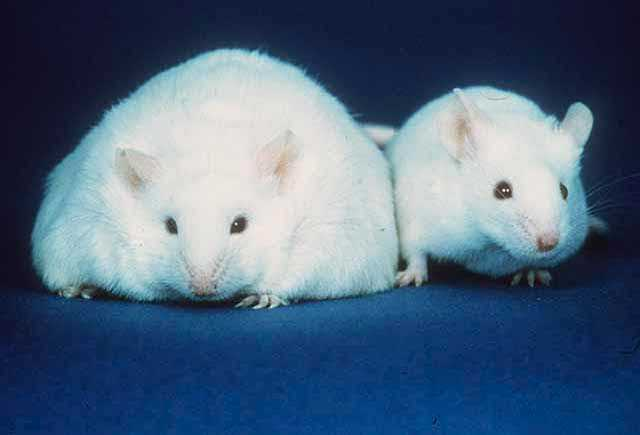
\includegraphics{Fatmouse}
\label{fig:ob_ob_mouse}
\caption{The ob/ob mouse (left), a laboratory mouse which has been genetically engineered to be obese, and an ordinary mouse (right). Photo from \parencite{commons2006}.}
\end{figure}

Our main goal in studying arguments is to separate the good ones from the bad ones. The argument about Clue we saw earlier is a good one, based on the process of elimination.  It is good because it leads to truth. If I've got all the premises right, the conclusion will also be right. The textbook \textit{Logic: Techniques of Formal Reasoning}\cite{Kalish1980} has a nice way of capturing the definition of logic: ``logic is the study of virtue in argument.'' \label{virtue_in_argument} This textbook essentially agrees with this definition, with the caveat that an argument is virtuous if it helps us get to the truth.

Logic is different from \textsc{\gls{rhetoric}}, which is the study of effective persuasion. Rhetoric does not look at virtue in argument. It only looks at the power of arguments, regardless of whether they lead to truth. An advertisement might convince you to buy a new truck by having a gravelly voiced announcer tell you it is ``ram tough'' and showing you a picture of the truck on top of a mountain, where it no doubt actually had to be airlifted. This sort of persuasion is often more effective at getting people to believe things than logical argument, but it has nothing to do with whether the truck is really the right thing to buy. In this textbook we will only be interested in rhetoric to the extent that we need to learn to defend ourselves against the misleading rhetoric of others. This will not, however, be anything close to a full treatment of the study of rhetoric.


%%%%%%%%%%%%%%%%%%%%%%%%%%%%%%%%%%%%%%%%%%%%%%%%%%%%%%%%%%%%%%%%%%%%%%%%%%%%%%%%%%%%%%%%%%%%%%%%%%%%%%%%%%%%%%%%%%%%%%%%%
% Statement, Argument, Premise, Conclusion
%%%%%%%%%%%%%%%%%%%%%%%%%%%%%%%%%%%%%%%%%%%%%%%%%%%%%%%%%%%%%%%%%%%%%%%%%%%%%%%%%%%%%%%%%%%%%%%%%%%%%%%%%%%%%%%%%%%%%%%%%

\section{Statement, Argument, Premise, Conclusion}\label{sec:partsofarguments}

So far we have defined logic as the study of argument and outlined its relationship to related fields. To go any further, we are going to need a more precise definition of what exactly an argument is. We have said that an argument is not simply two people disagreeing; it is an attempt to prove something using evidence. More specifically, an argument is composed of statements. In logic, we define a \textsc{\gls{statement}} \label{def:statement} as a unit of language that can be true or false. That means that statements are \textsc{\gls{truth evaluable}} \label{def:truth_evaluable}. All of the items below are statements.

\begin{enumerate}
	\item \label{itm:trex-true} \emph{Tyrannosaurus rex} went extinct 65 million years ago.
	\item \label{itm:trex-false} \emph{Tyrannosaurus rex} went extinct last week.
	\item \label{itm:trex-unknown} On this exact spot, 100  million years ago, a \emph{T. rex} laid a clutch of eggs.
	\item \label{itm:silly} Abraham Lincoln is the king of Mars.
	\item \label{itm:moral}Murder is wrong.
	\item \label{itm:opinion1}Abortion is murder.
	\item \label{itm:opinion2}Abortion is a woman's right.
	\item \label{itm:opinion3}Lady Gaga is pretty.
	\item \label{itm:definition}Murder is the unjustified killing of a person.
	\item \label{itm:nonsense}The slithy toves did gyre and gimble in the wabe.
	\item \label{itm:history}The murder of logician Richard Montague was never solved.
\end{enumerate}

Because a statement is something that can be true \emph{or} false, statements include truths like \ref{itm:trex-true} and falsehoods like \ref{itm:trex-false}.
A statement can also be something that that must either be true or false, but we don't know which, like \ref{itm:trex-unknown}.
A statement can be something that is completely silly, like \ref{itm:silly}.
Statements in logic include statements about morality, like \ref{itm:moral}, and things that in other contexts might be called ``opinions,'' like \ref{itm:opinion1} and \ref{itm:opinion2}.
People disagree strongly about whether \ref{itm:opinion1} or \ref{itm:opinion2} are true, but it is definitely possible for one of them to be true. The same is true about \ref{itm:opinion3}, although it is a less important issue than \ref{itm:opinion1} and \ref{itm:opinion2}.
A statement in logic can also simply give a definition, like \ref{itm:definition}.
This sort of statement announces that we plan to use words a certain way, which is different from statements that describe the world, like \ref{itm:trex-true}, or statements about morality, like \ref{itm:opinion1}.
Statements can include nonsense words like \ref{itm:nonsense}, because we don't really need to know what the statement is about to see that it is the sort of thing that can be true or false.
All of this relates back to the content neutrality of logic.
The statements we study can be about dinosaurs, abortion, Lady Gaga, and even the history of logic itself, as in statement \ref{itm:history}, which is true.

We are treating statements primarily as units of language or strings of symbols, and most of the time the statements you will be working with will just be words printed on a page. However, it is important to remember that statements are also what philosophers call ``speech acts.'' They are actions people take when they speak (or write). If someone makes a statement they are typically telling other people that they believe the statement to be true, and will back it up with evidence if asked to. When people make statements, they always do it in a context---they make statements at a place and a time with an audience. Often the context statements are made in will be important for us, so when we give examples, statements, or arguments we will sometimes include a description of the context. When we do that, we will give the context in \textit{italics}. See figure \ref{fig:statements_and_context} for examples. For the most part, the context for a statement or argument will be important in the chapters on critical thinking, when we are pursing the study of logic for practical reasons. In the chapters on formal logic, context is less important and we will be more likely to skip it.

\begin{figure*}
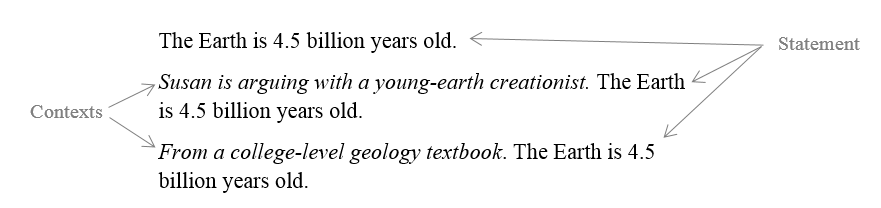
\includegraphics[width=\linewidth]{statement_and_contexts}
\caption{A statement in different contexts, or no context.}
\label{fig:statements_and_context}
\end{figure*}

``Statements'' in this text will \emph{not} include questions, commands, exclamations, or sentence fragments. Someone who asks a \emph{question} like ``Does the grass need to be mowed?'' is typically not claiming that anything is true or false. \emph{Questions} do not count as statements, but \emph{answers} usually will. ``What is this course about?'' is not a statement. An answer to that question such as ``No one knows what this course is about,'' is a statement.

For the same reason \emph{commands} do not count as statements for us. If someone bellows ``Mow the grass!'' they are not saying whether the grass has been mowed or not. You might infer that they believe the lawn has not been mowed, but then again maybe they think the lawn is fine and just want to see you exercise.

An exclamation like ``Ouch!'' is also neither true nor false. On its own, it is not a statement. We will treat ``Ouch, I hurt my toe!'' as meaning the same thing as ``I hurt my toe.'' The ``ouch'' does not add anything that could be true or false.

Finally, a lot of possible strings of words will fail to qualify as statements simply because they don't form a meaningful sentence. In your composition classes, these were probably referred to as sentence fragments. This includes strings of words that are parts of sentences, such as noun phrases like ``The tall man with the hat'' and verb phrases, like ``ran down the hall.'' Phrases like these are missing something they need to make a claim about the world. The class of sentence fragments also includes completely random combinations of words, like ``The up if blender route,'' which don't even have the form of a statement about the world.

Other logic textbooks describe the components of argument as ``propositions,'' or ``assertions,'' and we will use these terms sometimes as well.  There is actually a great deal of disagreement about what the differences between all of these things are and which term is best used to describe parts of arguments. However, none of that makes a difference for this textbook. Some textbooks will also use the term ``sentence'' here. We will not use the word ``sentence'' to mean the same thing as ``statement.'' Instead, we will use ``sentence'' the way it is used in ordinary grammar, to refer generally to statements, questions, and commands.

Sometimes the outward form of a speech act does not match how it is actually being used. A rhetorical question, for instance, has the outward form of a question, but is really a statement or a command. If someone says ``don't you think the lawn needs to be mowed?'' they may actually mean a statement like ``the lawn needs to be mowed'' or a command like ``mow the lawn, now.'' Similarly one might disguise a command as a statement. ``You will respect my authority'' \emph{is} either true or false---either you will or you will not. But the speaker may intend this as an order---''Respect me!''---rather than a prediction of how you will behave.

When we study argument, we need to express things as statements, because arguments are composed of statements. Thus if we encounter a rhetorical question while examining an argument, we need to convert it into a statement. ``Don't you think the lawn needs to be mowed'' will become ``the lawn needs to be mowed.'' Similarly, commands will become should statements. ``Mow the lawn, now!'' will need to be transformed into ``You should mow the lawn.''

The latter kind of change will be important in critical thinking, because critical thinking often studies arguments whose goal is to an get audience to do something. These are called \textsc{\glspl{practical argument}}\label{def:practical_argument}. Most advertising and political speech consists of practical arguments, and these are crucial topics for critical thinking.

Once we have a collection of statements, we can use them to build arguments. An \textsc{\gls{argument}} \label{def:argument} is a connected series of statements designed to convince an audience of another statement. Here an audience might be a literal audience sitting in front of you at some public speaking engagement. Or it might be the readers of a book or article. The audience might even be yourself as you reason your way through a problem. Let's start with an example of an argument given to an external audience. This passage is from an essay by Peter Singer called ``Famine, Affluence, and Morality'' in which he tries to convince people in rich nations that they need to do more to help people in poor nations who are experiencing famine.

\begin{quotation}
\noindent \textit{A contemporary philosopher writing in an academic journal.}
If it is in our power to prevent something bad from happening, without thereby sacrificing anything of comparable moral importance, we ought, morally, to do so. Famine is something bad, and it can be prevented without sacrificing anything of comparable moral importance. So, we ought to prevent famine.\cite{Singer1972}  
\end{quotation}\label{singer_quote}

Singer wants his readers to work to prevent famine. This is represented by the last statement of the passage, ``we ought to prevent famine,'' which is called the conclusion of the passage. The \textsc{\gls{conclusion}} of an argument is the statement that the argument is trying to convince the audience of. The statements that do the convincing are called the \textsc{\glspl{premise}}. In this case, the argument has three premises: (1) ``If it is in our power to prevent something bad from happening, without thereby sacrificing anything of comparable moral importance, we ought, morally, to do so''; (2) ``Famine is something bad''; and (3) ``it can be prevented without sacrificing anything of comparable moral importance.''

Now let's look at an example of internal reasoning.

\begin{quotation}
	\noindent\textit{Jack arrives at the track, in bad weather.} There is no one here. I guess the race is not happening. \label{racetrack}
\end{quotation}

In the passage above, the words in \textit{italics} explain the context for the reasoning, and the words in regular type represent what Jack is actually thinking to himself.
(We will talk more about his way of representing reasoning in section \ref{sec:arguments_and_nonarguments}, below.)
This passage again has a premise and a conclusion. The premise is that no one is at the track, and the conclusion is that the race was canceled. The context gives another reason why Jack might believe the race has been canceled, the weather is bad. You could view this as another premise---it is very likely a reason Jack has come to believe that the race is canceled. In general, when you are looking at people's internal reasoning, it is often hard to determine what is actually working as a premise and what is just working in the background of their unconscious.


When people give arguments to each other, they typically use words like ``therefore'' and ``because.'' These are meant to signal to the audience that what is coming is either a premise or a conclusion in an argument. Words and phrases like ``because'' signal that a premise is coming, so we call these \textsc{\glspl{premise indicator}}. Similarly, words and phrases like ``therefore'' signal a conclusion and are called \textsc{\glspl{conclusion indicator}}. The argument from Peter Singer (on page \pageref{singer_quote}) uses the conclusion indicator word, ``so.'' Table \ref{tab:indicators} is an incomplete list of indicator words and phrases in English.


\begin{table}
\begin{longtabu} to \textwidth {X[4,p]X[8,p]}
\textbf{Premise Indicators:} & because, as, for, since, given that, for the reason that \\
& \\
\textbf{Conclusion Indicators:} & therefore, thus, hence, so, consequently, it follows that, in conclusion, as a result, then, must, accordingly, this implies that, this entails that, we may infer that \\
\end{longtabu}
\caption{Premise and Conclusion Indicators.}
\label{tab:indicators}
\end{table}

The two passages we have looked at in this section so far have been simply presented as quotations. But often it is extremely useful to rewrite arguments in a way that makes their logical structure clear. One way to do this is to use something called standard or ``canonical form.'' An argument written in \textsc{\gls{canonical form}} \label{def:canonical_form} has each premise numbered and written on a separate line.\footnote{This is also called standard form. We will use both terms throughout the textbook.} Indicator words and other unnecessary material should be removed from the premises. Although you can shorten the premises and conclusion, you need to be sure to keep them all complete sentences with the same meaning, so that they can be true or false. The argument from Peter Singer, above, looks like this in canonical form:

\begin{kormanize}
\premise{If we can stop something bad from happening, without sacrificing anything of comparable moral importance, we ought to do so.}
\premise{Famine is something bad.}
\premise{Famine can be prevented without sacrificing anything of comparable moral importance.}
\conclusion{We ought to prevent famine.}
\end{kormanize}

Each statement has been written on its own line and given a number. The statements have been paraphrased slightly, for brevity, and the indicator word ``so'' has been removed. Also notice that the ``it'' in the third premise has been replaced by the word ``famine,'' so that statements reads naturally on its own.

Similarly, we can rewrite the argument Jack gives at the racetrack, on page \pageref{racetrack}, like this:

\begin{kormanize}
\premise{There is no one at the race track.}
\conclusion{ The race is not happening.}
\end{kormanize}

Notice that we did not include anything from the part of the passage in italics. The italics represent the context, not the argument itself. Also, notice that the ``I guess'' has been removed. When we write things out in canonical form, we write the content of the statements, ignore information about the speaker's mental state, like ``I believe'' or ``I guess.''

One of the first things you have to learn to do in logic is to identify arguments and rewrite them in canonical form. This is a foundational skill for everything else we will be doing in this text, so we are going to run through a few examples now, and there will be more in the exercises. The passage below is paraphrased from the ancient Greek philosopher Aristotle.

\begin{quotation}\noindent \textit{An ancient philosopher, writing for his students} Again, our observations of the stars make it evident that the earth is round. For quite a small change of position to south or north causes a manifest alteration in the stars which are overhead. (\cite{Aristotle:heavens}, 298a2-10)
\label{on_the_heavens} \end{quotation}

The first thing we need to do to put this argument in canonical form is to identify the conclusion. The indicator words are the best way to do this. The phrase ``make it evident that'' is a conclusion indicator phrase. He is saying that everything else is \textit{evidence} for what follows. So we know that the conclusion is that the earth is round. ``For'' is a premise indicator word---it is sort of a weaker version of ``because.''  Thus the premise is that the stars in the sky change if you move north or south. In canonical form, Aristotle's argument that the earth is round looks like this.\\


\begin{kormanize}
\premise{There are different stars overhead in the northern and southern parts of the earth.}
\conclusion{ The earth is spherical in shape.}
\end{kormanize}

That one is fairly simple, because it just has one premise. Here's another example of an argument, this time from the book of Ecclesiastes in the Bible. The speaker in this part of the bible is generally referred to as The Preacher, or in Hebrew, Koheleth. In this verse, Koheleth uses both a premise indicator and a conclusion indicator to let you know he is giving reasons for enjoying life.

\begin{quotation}
\noindent \textit{The words of the Preacher, son of David, King of Jerusalem} There is something else meaningless that occurs on earth: the righteous who get what the wicked deserve, and the wicked who get what the righteous deserve. \ldots So I commend the enjoyment of life, because there is nothing better for a person under the sun than to eat and drink and be glad. (Ecclesiastes 8:14-15, New International Version)
\end{quotation}

Koheleth begins by pointing out that good things happen to bad people and bad things happen to good people. This is his first premise. (Most Bible teachers provide some context here by pointing that that the ways of God are mysterious and this is an important theme in Ecclesiastes.) Then Koheleth gives his conclusion, that we should enjoy life, which he marks with the word ``so.'' Finally he gives an extra premise, marked with a ``because,'' that there is nothing better for a person than to eat and drink and be glad. In canonical form, the argument would look like this.


\begin{kormanize}
\premise{Good things happen to bad people and bad things happen to good people.}
\premise{There is nothing better for people than to eat, to drink and to enjoy life.}
\conclusion{You should enjoy life.}
\end{kormanize}

Notice that in the original passages, Aristotle put the conclusion in the first sentence, while Koheleth put it in the middle of the passage, between two premises. In ordinary English, people can put the conclusion of their argument where ever they want. However, when we write the argument in canonical form, the conclusion goes last.

Unfortunately, indicator words aren't a perfect guide to when people are giving an argument. Look at this passage from a newspaper:

\begin{quotation}
\noindent \textit{From the general news section of a national newspaper} The new budget underscores the consistent and paramount importance of tax cuts in the Bush philosophy. His first term cuts affected more money than any other initiative undertaken in his presidency, including the costs thus far of the war in Iraq. All told, including tax incentives for health care programs and the extension of other tax breaks that are likely to be taken up by Congress, the White House budget calls for nearly \$300 billion in tax cuts over the next five years, and \$1.5 trillion over the next 10 years.  \cite{Toner2006}
\end{quotation}

Although there are no indicator words, this is in fact an argument. The writer wants you to believe something about George Bush: tax cuts are his number one priority. The next two sentences in the paragraph give you reasons to believe this. You can write the argument in canonical form like this.

\begin{kormanize}
\premise{Bush's first term cuts affected more money than any other initiative undertaken in his presidency, including the costs thus far of the war in Iraq.}
\premise{The White House budget calls for nearly \$300 billion in tax cuts over the next five years, and \$1.5 trillion over the next 10 years.}
\conclusion{Tax cuts are of consistent and paramount importance of in the Bush philosophy.}
\end{kormanize}

The ultimate test of whether something is an argument is simply whether some of the statements provide reason to believe another one of the statements. If some statements support others, you are looking at an argument. The speakers in these two cases use indicator phrases to let you know they are trying to give an argument.

A final bit of terminology for this section. An \textsc{\gls{inference}} \label{def:Inference} is the act of coming to believe a conclusion on the basis of some set of premises. When Jack in the example above saw that no one was at the track, and came to believe that the race was not on, he was making an inference. We also use the term inference to refer to the connection between the premises and the conclusion of an argument. If your mind moves from premises to conclusion, you make an inference, and the premises and the conclusion are said to be linked by an inference. In that way inferences are like argument glue: they hold the premises and conclusion together.



%%%%%%%%%%%%%%%%%%%%%%%%%%%%%%%%%%%%%%%%%%%%%%%%%%%%%%%%%%%%%%%%%%%%%%%%%%%%%%%%
% Arguments and Nonarguments
%%%%%%%%%%%%%%%%%%%%%%%%%%%%%%%%%%%%%%%%%%%%%%%%%%%%%%%%%%%%%%%%%%%%%%%%%%%%%%%%

\section{Arguments and Nonarguments}\label{sec:arguments_and_nonarguments}

We just saw that arguments are made of statements. However, there are lots of other things you can do with statements. Part of learning what an argument is involves learning what an argument is not, so in this section and the next we are going to look at some other things you can do with statements besides make arguments.

The list below of kinds of nonarguments is not meant to be exhaustive: there are all sorts of things you can do with statements that are not discussed. Nor are the items on this list meant to be exclusive. One passage may function as both, for instance, a narrative and a statement of belief. Right now we are looking at real world reasoning, so you should expect a lot of ambiguity and imperfection.

\subsection{Simple Statements of Belief}

An argument is an attempt to persuade an audience to believe something, using reasons. Often, though, when people try to persuade others to believe something, they skip the reasons, and give a \textsc{\gls{simple statement of belief}}. \label{def:simple_statement_of_belief} This is a kind of nonargumentative passage where the speaker simply asserts what they believe without giving reasons. Sometimes simple statements of belief are prefaced with the words ``I believe,'' and sometimes they are not. A simple statements of belief can be a profoundly inspiring way to change people's hearts and minds. Consider this passage from Dr. Martin Luther King's Nobel acceptance speech.

\begin{quotation} \noindent I believe that even amid today's mortar bursts and whining bullets, there is still hope for a brighter tomorrow. I believe that wounded justice, lying prostrate on the blood-flowing streets of our nations, can be lifted from this dust of shame to reign supreme among the children of men. I have the audacity to believe that peoples everywhere can have three meals a day for their bodies, education and culture for their minds, and dignity, equality and freedom for their spirits. \cite{King2001} \end{quotation}

This actually is a part of a longer passage that consists almost entirely of statements that begin with some variation of ``I believe.''It is incredibly powerful oration, because the audience, feeling the power of King's beliefs, comes to share in those beliefs. The language King uses to describe how he believes is important, too. He says his belief in freedom and equality requires audacity, making the audience feel his courage and want to share in this courage by believing the same things.

These statements are moving, but they do not form an argument. None of these statements provide evidence for any of the other statements. In fact, they all say roughly the same thing, that good will triumph over evil. So the study of this kind of speech belongs to the discipline of rhetoric, not of logic.

\subsection{Expository Passages}

Perhaps the most basic use of a statement is to convey information. Often if we have a lot of information to convey, we will sometimes organize our statements around a theme or a topic. Information organized in this fashion can often appear like an argument, because all of the statements in the passage relate back to some central statement. However, unless the other statements are given as reasons to believe the central statement, the passage you are looking at is not an argument. Consider this passage:

\begin{quotation}\noindent\textit{From a college psychology textbook.} Eysenck advocated three major behavior techniques that have been used successfully to treat a variety of phobias. These techniques are modeling, flooding, and systematic desensitization. In \textbf{modeling} phobic people watch nonphobics cope successfully with dreaded objects or situations.In \textbf{flooding} clients are exposed to dreaded objects or situations for prolonged periods of time in order to extinguish their fear. In contrast to flooding, \textbf{systematic desensitization} involves gradual, client-controlled exposure to the anxiety eliciting object or situation. (Adapted from Ryckman \cite{Ryckman2007}) \end{quotation}

We call this kind of passage an expository passage. In an \textsc{\gls{expository passage}}, \label{def:expository_passage} statements are organized around a central theme or topic statement. The topic statement might look like a conclusion, but the other statements are not meant to be evidence for the topic statement. Instead, they elaborate on the topic statement by providing more details or giving examples. In the passage above, the topic statement is ``Eysenck advocated three major behavioral techniques \ldots.'' The statements describing these techniques elaborate on the topic statement, but they are not evidence for it. Although the audience may not have known this fact about Eysenk before reading the passage, they will typically accept the truth of this statement instantly, based on the textbook's authority. Subsequent statements in the passage merely provide detail.

Deciding whether a passage is an argument or an expository passage is complicated by the fact that sometimes people argue by example:

\begin{longtabu} to \textwidth {X[3,p]X[8,p]}
\textbf{Steve:} & Kenyans are better distance runners than everyone else. \\
\textbf{Monica:} & Oh come on, that sounds like an exaggeration of a stereotype that isn't even true.\\
\textbf{Steve:} & What about Dennis Kimetto, the Kenyan who set the world record for running the marathon? And you know who the previous record holder was: Emmanuel Mutai, also Kenyan. \\
\end{longtabu}

Here Steve has made a general statement about all Kenyans. Monica clearly doubts this claim, so Steve backs it up with some examples that seem to match his generalization. This isn't a very strong way to argue: moving from two examples to statement about all Kenyans is probably going to be a kind of bad argument known as a hasty generalization. (This mistake is covered in the complete version of this text in the chapter on induction Chapter~\ref{ch:inductivelogic} on induction.) The point here however, is that Steve is just offering it as an argument.

The key to telling the difference between expository passages and arguments by example is whether there is a conclusion that they audience needs to be convinced of. In the passage from the psychology textbook, ``Eysenck advocated three major behavioral techniques'' doesn't really work as a conclusion for an argument. The audience, students in an introductory psychology course, aren't likely to challenge this assertion, the way Monica  challenges Steve's overgeneralizing claim.

Context is very important here, too. The Internet is a place where people argue in the ordinary sense of exchanging angry words and insults. In that context, people are likely to actually give some arguments in the logical sense of giving reasons to believe a conclusion.

\subsection{Narratives}

Statements can also be organized into descriptions of events and actions, as in this snippet from book V of \textit{Harry Potter}.

\begin{quotation} \noindent But she [Hermione] broke off; the morning post was arriving and, as usual, the \textit{Daily Prophet} was soaring toward her in the beak of a screech owl, which landed perilously close to the sugar bowl and held out a leg. Hermione pushed a Knut into its leather pouch, took the newspaper, and scanned the front page critically as the owl took off again. \cite{Rowling2003} \end{quotation}

We will use the term \textsc{\gls{narrative}} \label{def:narrative} loosely to refer to any passage that gives a sequence of events or actions. A narrative can be fictional or nonfictional. It can be told in regular temporal sequence or it can jump around, forcing the audience to try to reconstruct a temporal sequence. A narrative can describe a short sequence of actions, like Hermione taking a newspaper from an owl, or a grand sweep of events, like this passage about the  rise and fall of an empire in the ancient near east:

\begin{quotation}
The Guti were finally expelled from Mesopotamia by the Sumerians of Erech (\textit{c}. 2100), but it was left to the kings of Ur's famous third dynasty to re-establish the Sargonoid frontiers and write the final chapter of the Sumerian History. The dynasty lasted through the twenty first century at the close of which the armies of Ur were overthrown by the Elamites and Amorites \cite{McEvedy1967}.
\end{quotation}

This passage does not feature individual people performing specific actions, but it is still united by character and action. Instead of Hermione at breakfast, we have the Sumarians in Mesopotamia. Instead of retrieving a message from an owl, the conquer the Guti, but then are conquered by the Elamites and Amorites. The important thing is that the statements in a narrative are not related as premises and conclusion. Instead, they are all events which are united common characters acting in specific times and places.

\subsection{Socratic Elenchus}

Now we will consider one example of a collection of sentences that \emph{is} an argument: the Socratic elenchus.

The Greek philosopher Socrates was known for his odd style of arguing with his interlocutors. While Socrates himself left no known writings, his students Plato and Xenophon wrote many dialogues (essentially, lengthy academic stories or plays) in which Socrates was a main character. The character Socrates and the actual person Socrates are thought to have much in common (although this is still an object of much academic debate).

In many of the dialogues, Socrates engages his interlocutors (that is, his conversational and argumentative partners) in what is called the \textsc{\Gls{socratic elenchus}} \label{def:socraticelenchus} in order to demonstrate that their previously-held beliefs were false or contradictory. The elenchus is a style of argumentation in which two statements (usually definitions) are shown to be contradictory by means of critical questioning, so an alternative is sought.

For example, Socrates discusses the nature of piety with Euthyphro and asks Euthyphro whether pious actions are loved by the gods. Euthyphro, of course, answers in the affirmative. Socrates then asks whether pious actions are \emph{made pious} by the gods' love or if the gods just so happen to love piety. Euthyphro is unsure, since he is not certain what \emph{makes} pious actions pious in the first place. If the gods \emph{make} those actions pious, Socrates reasons, then they could just as easily have mande any actions whatsoever pious. However, if the gods simply love piety as it is, then this seems to detract from the power of the gods. After all, the gods would have no say in what they find good!

This is just one example of the Socratic elenchus.

\section*{Key Terms}
\begin{fullwidth}
\begin{multicols}{2}
\begin{sortedlist}
\sortitem{Logic}{}
\sortitem{Metareasoning}{}
\sortitem{Metacognition}{}
\sortitem{Content neutrality}{}
\sortitem{Formal logic}{}
\sortitem{Critical thinking}{}
\sortitem{Informal logic}{}
\sortitem{Rhetoric}{}
\sortitem{Canonical form}{}
\sortitem{Conclusion indicator}{}
\sortitem{Premise indicator}{}
\sortitem{Statement}{}
\sortitem{Argument}{}
\sortitem{Conclusion}{}
\sortitem{Premise}{}
\sortitem{Inference}{}
\sortitem{Simple statement of belief}{}
\sortitem{Expository passage}{}
\sortitem{Narrative}{}
\sortitem{Explanation}{}
\sortitem{Reason}{}
\sortitem{Target proposition}{}
\sortitem{Critical thinker}{}
\sortitem{Practical argument}{}
\sortitem{Socratic elenchus}{}
\end{sortedlist}
\end{multicols}
\end{fullwidth}
